% Slides for 2025-08-26
% To create a slide, use the following:
% \begin{frame}{TITLE}
%     BODY
% \end{frame}

% To create a slide with a bullet list, use the following:
% \begin{frame}{TITLE}
%     \begin{itemize}
%         \item ITEM 1
%         \item ITEM 2
%     \end{itemize}    
% \end{frame}

% To create a slide with numbered list, use the following:
% \begin{frame}{TITLE}
%     \begin{enumerate}
%         \item ITEM 1
%         \item ITEM 2
%     \end{enumerate}
% \end{frame}

% To create a slide with a graphic:
% 1. Add the graphic to this folder (named picture.png)
% 2. Use the following:
% \begin{frame}{TITLE}
%     \centering
%     \includegraphics[height=0.7\textheight,width=0.7\textwidth,keepaspectratio]{picture.png}
% \end{frame}

% To create a slide with two columns, use the following:
% \begin{frame}{TITLE}
%     \begin{columns}
%         \begin{column}{0.5\textwidth}
%             COLUMN 1 BODY
%         \end{column}
%         \begin{column}{0.5\textwidth}
%             COLUMN 2 BODY
%         \end{column}
%     \end{columns}
% \end{frame}

\begin{frame}{Auto Laser Calibration}
    \begin{itemize}
      \item Derived a solution that does not require calibration images 
      \item Simplifies processing and diving!
    \end{itemize}
\end{frame}

\begin{frame}{Strength in Numbers?}
  \begin{columns}
    \begin{column}{0.3\textwidth}
      \begin{itemize}
        \item LR and $R^2$
        \item ODR and MSE
        \item Mahalanoblis and $\chi^2$
      \end{itemize}
    \end{column}

    \begin{column}{0.7\textwidth}
      \raggedright    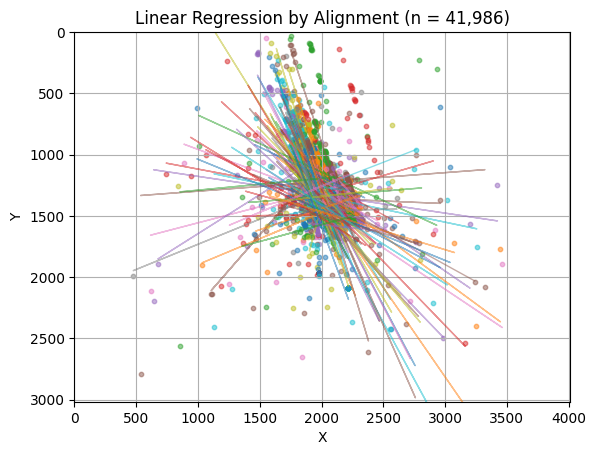
\includegraphics[height=0.7\textheight,keepaspectratio]{images/regression.png}
    \end{column}
  \end{columns}
\end{frame}

\begin{frame}{Depth Is All You Need}
    \centering
    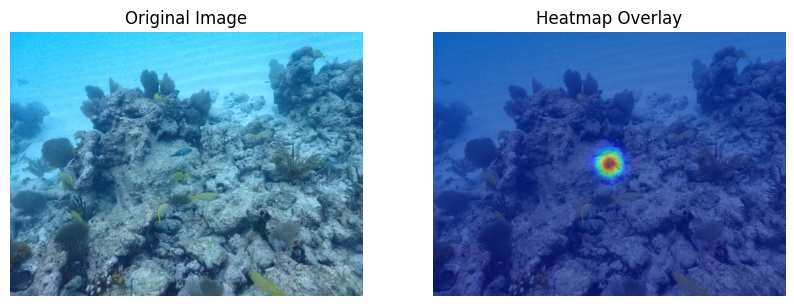
\includegraphics[height=0.95\textheight,width=0.95\textwidth,keepaspectratio]{images/bullseye.png}
\end{frame}

\begin{frame}{Depth Anything Anything}
    \centering
    \includegraphics[height=0.95\textheight,width=0.95\textwidth,keepaspectratio]{images/detection.png}
\end{frame}

\begin{frame}{Perhaps You Can Tuna Fish}
    \centering
    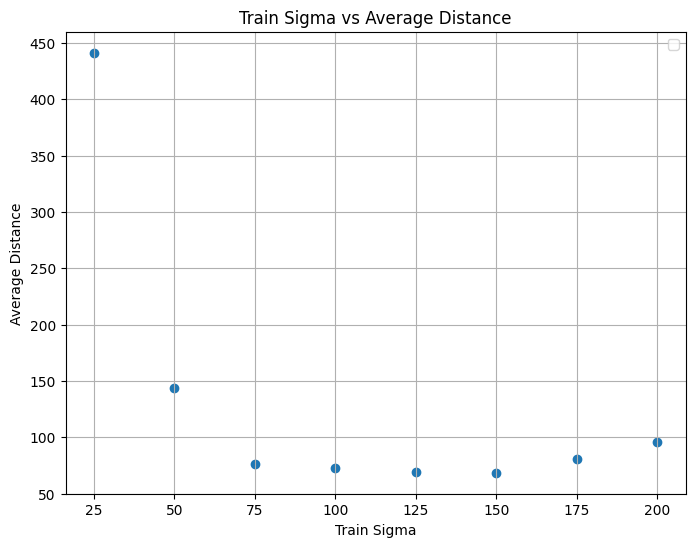
\includegraphics[height=0.95\textheight,width=0.95\textwidth,keepaspectratio]{images/tuning.png}
\end{frame}

\begin{frame}{LiDAR SLAM}
    \begin{itemize}
        \item LiDAR SLAM combines multiple angles for better accuracy
    \end{itemize}

    \centering
    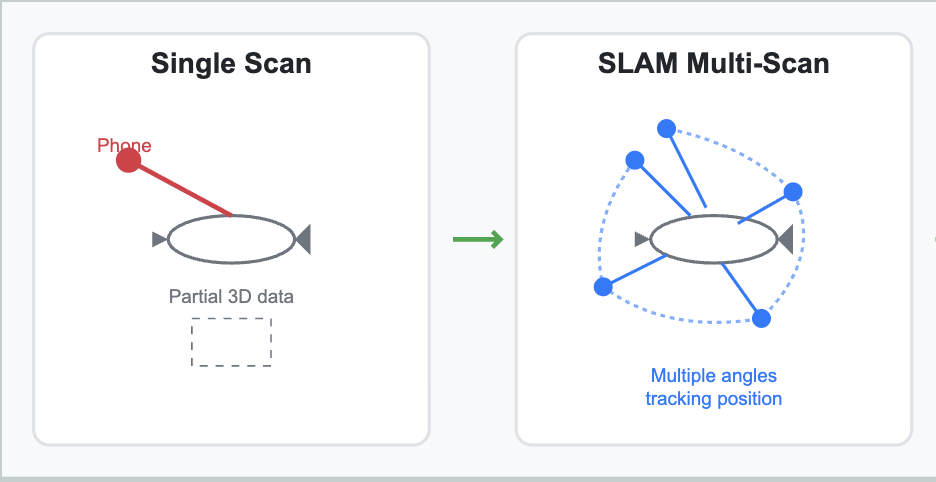
\includegraphics[height=0.7\textheight,keepaspectratio]{images/LiDAR SLAM.png}
\end{frame}


\begin{frame}{Current Set Up}
    \centering
    \includegraphics[height=0.95\textheight,keepaspectratio]{images/vertical_pi.png}
\end{frame}

\begin{frame}{It's getting hot in here}
    \centering
    \includegraphics[height=0.95\textheight,width=0.45\textwidth,keepaspectratio]{images/pool_stress_test.png}
    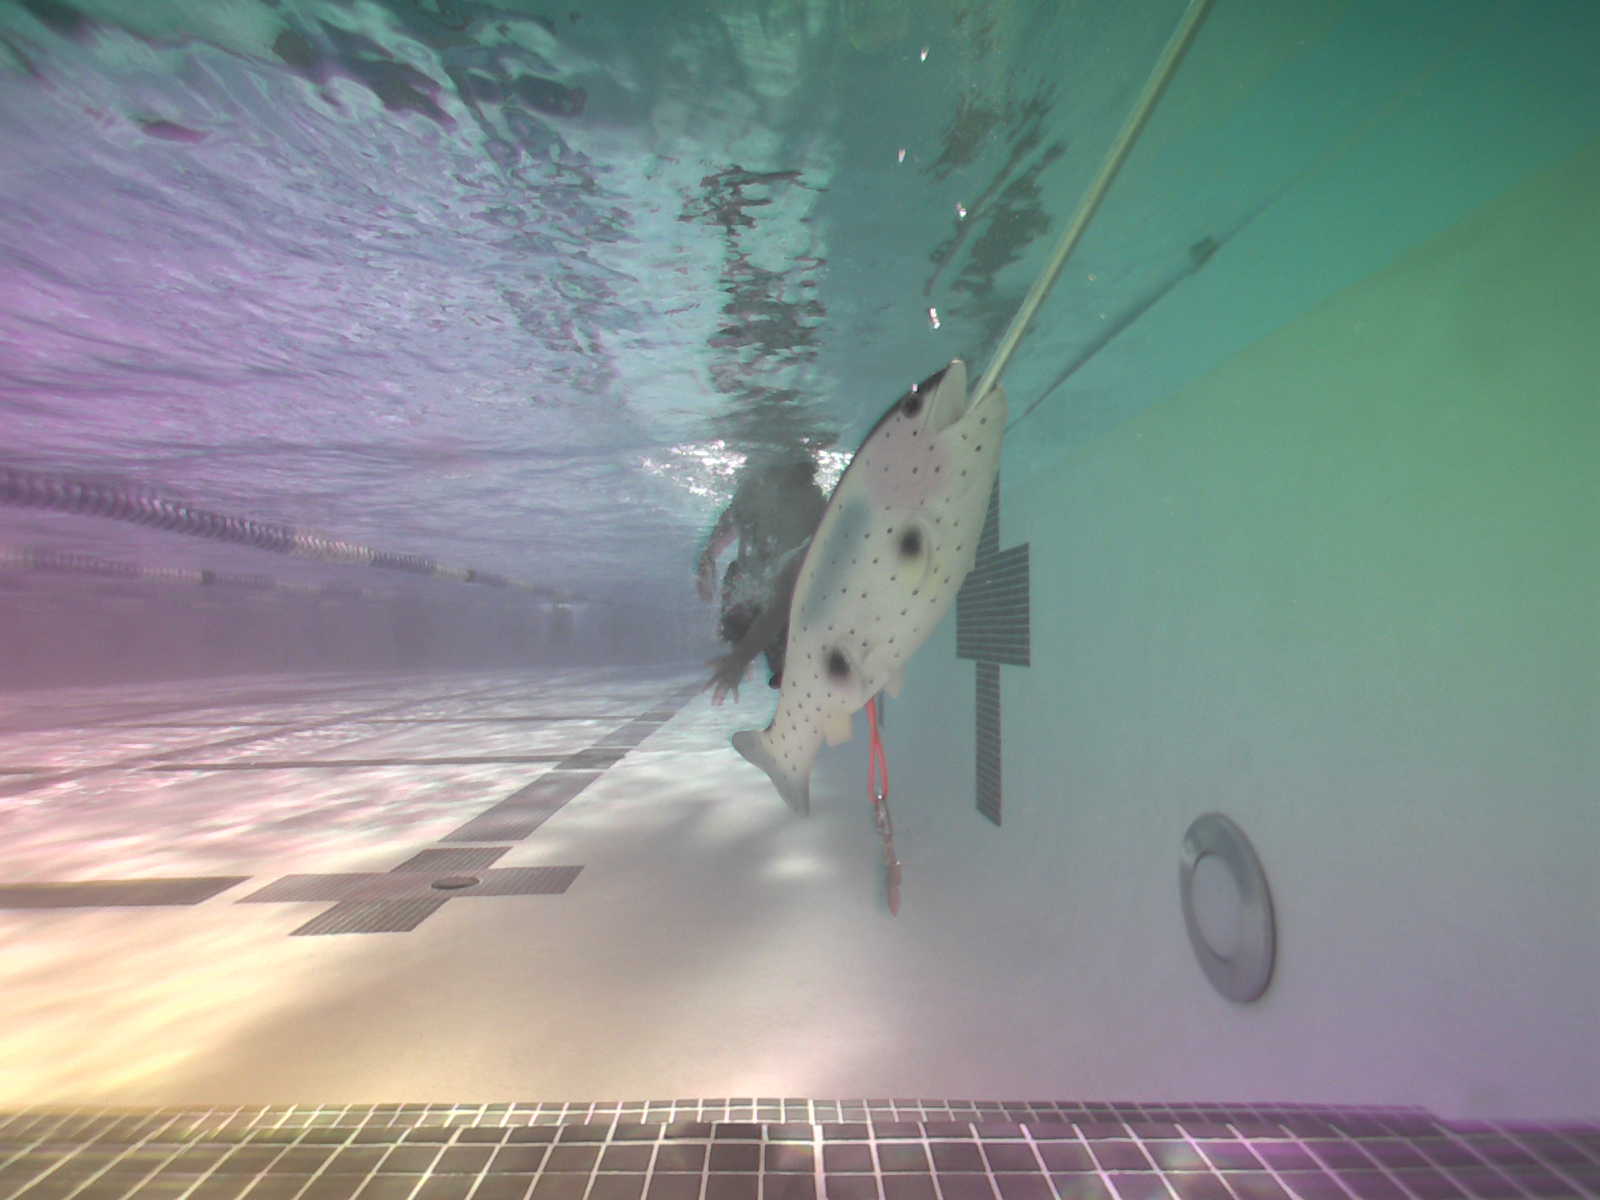
\includegraphics[height=0.95\textheight,width=0.45\textwidth,keepaspectratio]{images/ginny_rubik_pi.png}
\end{frame}

\begin{frame}{Whoops...}
    \centering
    \includegraphics[height=0.95\textheight,width=0.5\textwidth,keepaspectratio]{images/wrong_pad_placement.png}
    \includegraphics[height=0.95\textheight,width=0.5\textwidth,keepaspectratio]{images/correct_pad_placement.png}
\end{frame}

\begin{frame}{Results!}
    \centering
    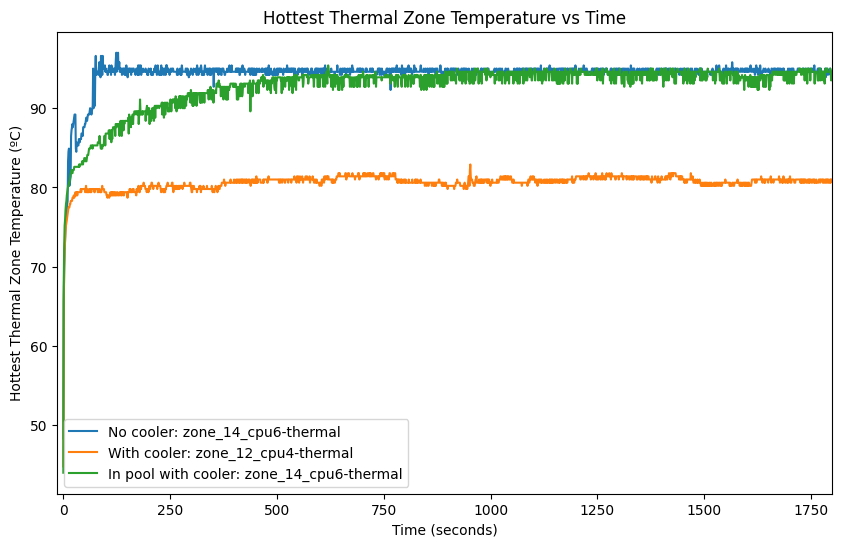
\includegraphics[height=0.95\textheight,width=0.95\textwidth,keepaspectratio]{images/hottest_zone_comparison.png}
\end{frame}

\begin{frame}{Looking Closer}
    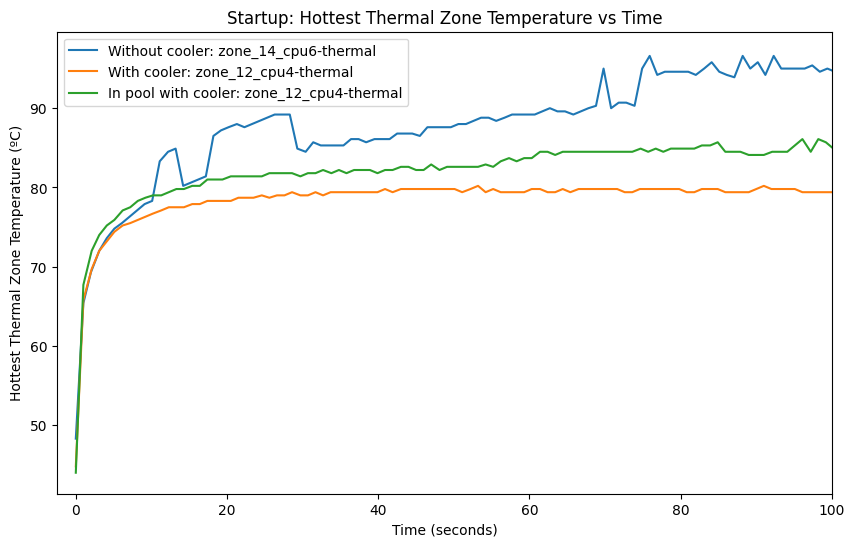
\includegraphics[width=0.95\textwidth,keepaspectratio]{images/startup_hottest_zone.png}
\end{frame}

\begin{frame}{Further Along}
    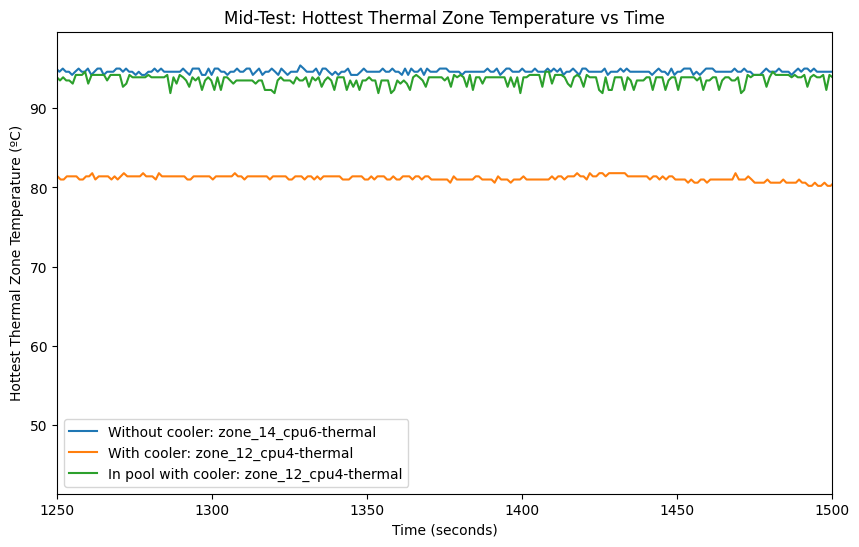
\includegraphics[width=0.95\textwidth,keepaspectratio]{images/mid-test_hottest_zone.png}
\end{frame}

\begin{frame}{Throttling?}
    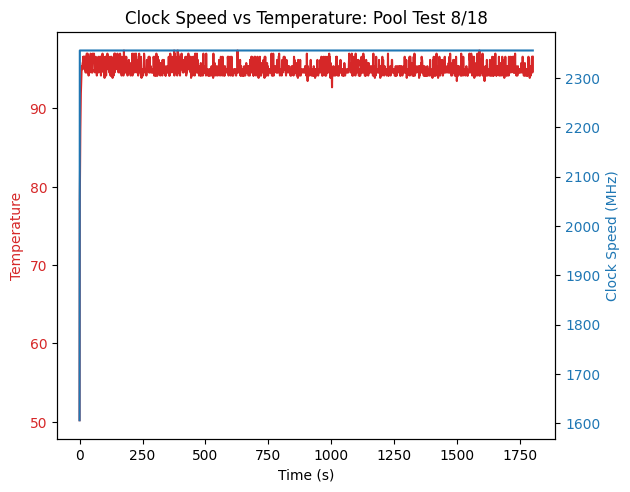
\includegraphics[width=0.3\textwidth,keepaspectratio]{images/clock_speed_8-18.png}
    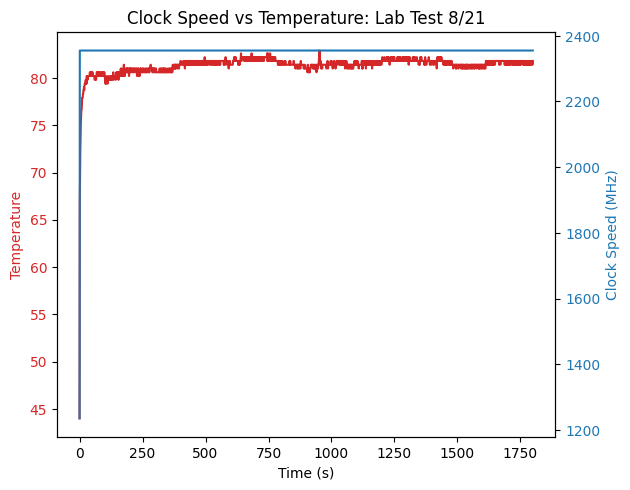
\includegraphics[width=0.3\textwidth,keepaspectratio]{images/clock_speed_8-21.png}
    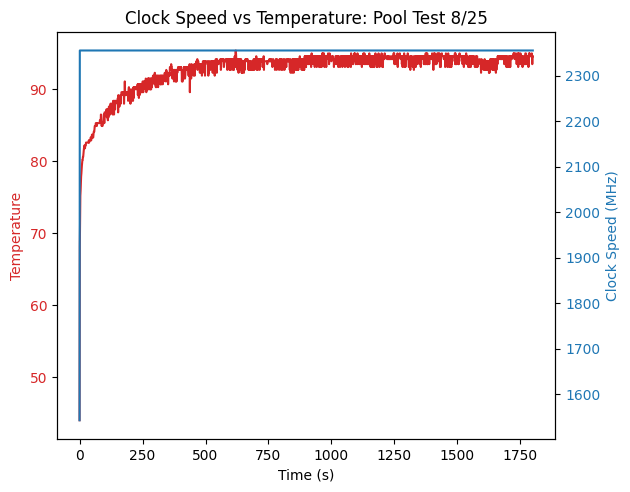
\includegraphics[width=0.3\textwidth,keepaspectratio]{images/clock_speed_8-25.png}
\end{frame}

\begin{frame}{What next?}
    \begin{columns}
        \begin{column}{0.5\textwidth}
            \begin{itemize}
                \item Aluminum: 109.33 W, 0.1004 kg
                \item Copper: 179.91 W, 0.4145 kg
            \end{itemize}
        \end{column}
        \begin{column}{0.5\textwidth}
            \includegraphics[height=0.55\textheight,keepaspectratio]{images/horizontal_pi.png}
        \end{column}
    \end{columns}
\end{frame}
